%!TeX root=../pridetop.tex
\chapter[Chapter \thechapter]{}
	
	\begin{figure}[t!]
\centering
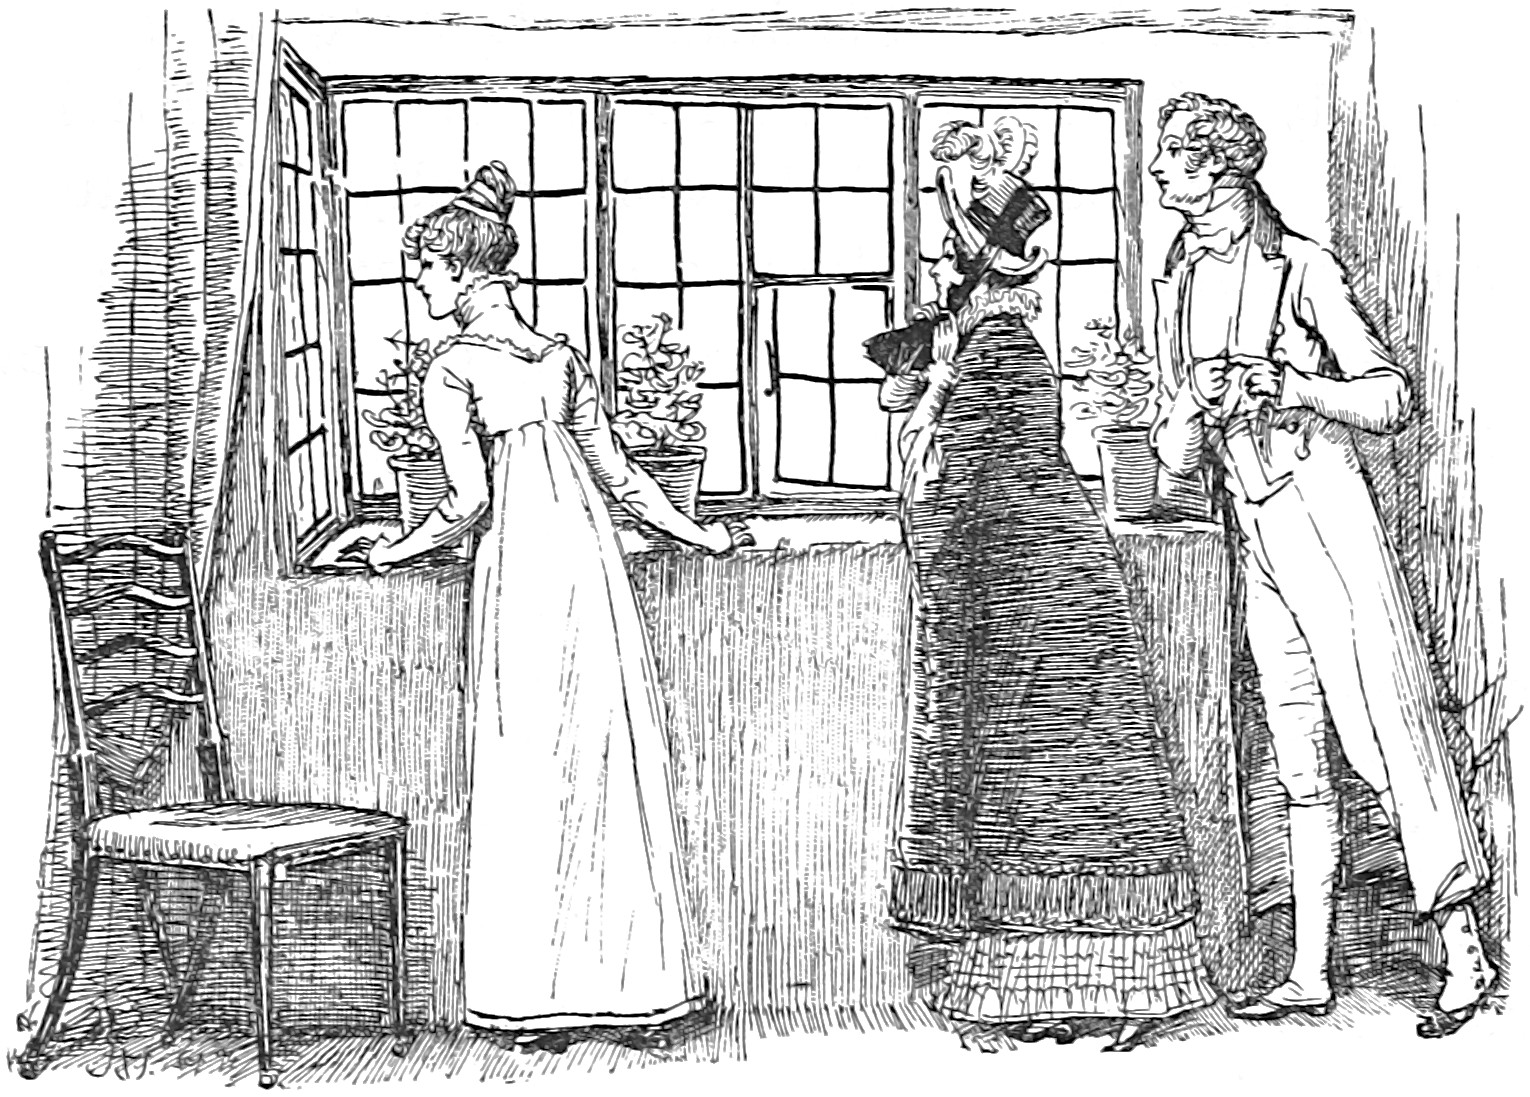
\includegraphics[width=\linewidth]{44top}
\captionlistentry{Headpiece to Chapter \thechapter}
\end{figure}


\lettrine[lines=6,image=true]{initials/chap44e}{lizabeth}  had settled it that Mr Darcy would bring his sister to visit her the very day after her reaching Pemberley; and was, consequently, resolved not to be out of sight of the inn the whole of that morning. But her conclusion was false; for on the very morning after their own arrival at Lambton these visitors came. They had been walking about the place with some of their new friends, and were just returned to the inn to dress themselves for dining with the same family, when the sound of a carriage drew them to a window, and they saw a gentleman and lady in a curricle driving up the street. Elizabeth, immediately recognizing the livery, guessed what it meant, and imparted no small degree of surprise to her relations, by acquainting them with the honour which she expected. Her uncle and aunt were all amazement; and the embarrassment of her manner as she spoke, joined to the circumstance itself, and many of the circumstances of the preceding day, opened to them a new idea on the business. Nothing had ever suggested it before, but they now felt that there was no other way of accounting for such attentions from such a quarter than by supposing a partiality for their niece. While these newly-born notions were passing in their heads, the perturbation of Elizabeth's feelings was every moment increasing. She was quite amazed at her own discomposure; but, amongst other causes of disquiet, she dreaded lest the partiality of the brother should have said too much in her favour; and, more than commonly anxious to please, she naturally suspected that every power of pleasing would fail her.

She retreated from the window, fearful of being seen; and as she walked up and down the room, endeavouring to compose herself, saw such looks of inquiring surprise in her uncle and aunt as made everything worse.

Miss Darcy and her brother appeared, and this formidable introduction took place. With astonishment did Elizabeth see that her new acquaintance was at least as much embarrassed as herself. Since her being at Lambton, she had heard that Miss Darcy was exceedingly proud; but the observation of a very few minutes convinced her that she was only exceedingly shy. She found it difficult to obtain even a word from her beyond a monosyllable.

Miss Darcy was tall, and on a larger scale than Elizabeth; and, though little more than sixteen, her figure was formed, and her appearance womanly and graceful. She was less handsome than her brother, but there was sense and good-humour in her face, and her manners were perfectly unassuming and gentle. Elizabeth, who had expected to find in her as acute and unembarrassed an observer as ever Mr Darcy had been, was much relieved by discerning such different feelings.

They had not been long together before Darcy told her that Bingley was also coming to wait on her; and she had barely time to express her satisfaction, and prepare for such a visitor, when Bingley's quick step was heard on the stairs, and in a moment he entered the room. All Elizabeth's anger against him had been long done away; but had she still felt any, it could hardly have stood its ground against the unaffected cordiality with which he expressed himself on seeing her again. He inquired in a friendly, though general, way, after her family, and looked and spoke with the same good-humoured ease that he had ever done.

To Mr and Mrs Gardiner he was scarcely a less interesting personage than to herself. They had long wished to see him. The whole party before them, indeed, excited a lively attention. The suspicions which had just arisen of Mr Darcy and their niece, directed their observation towards each with an earnest, though guarded, inquiry; and they soon drew from those inquiries the full conviction that one of them at least knew what it was to love. Of the lady's sensations they remained a little in doubt; but that the gentleman was overflowing with admiration was evident enough.

\begin{figure}[tbh]
\centering
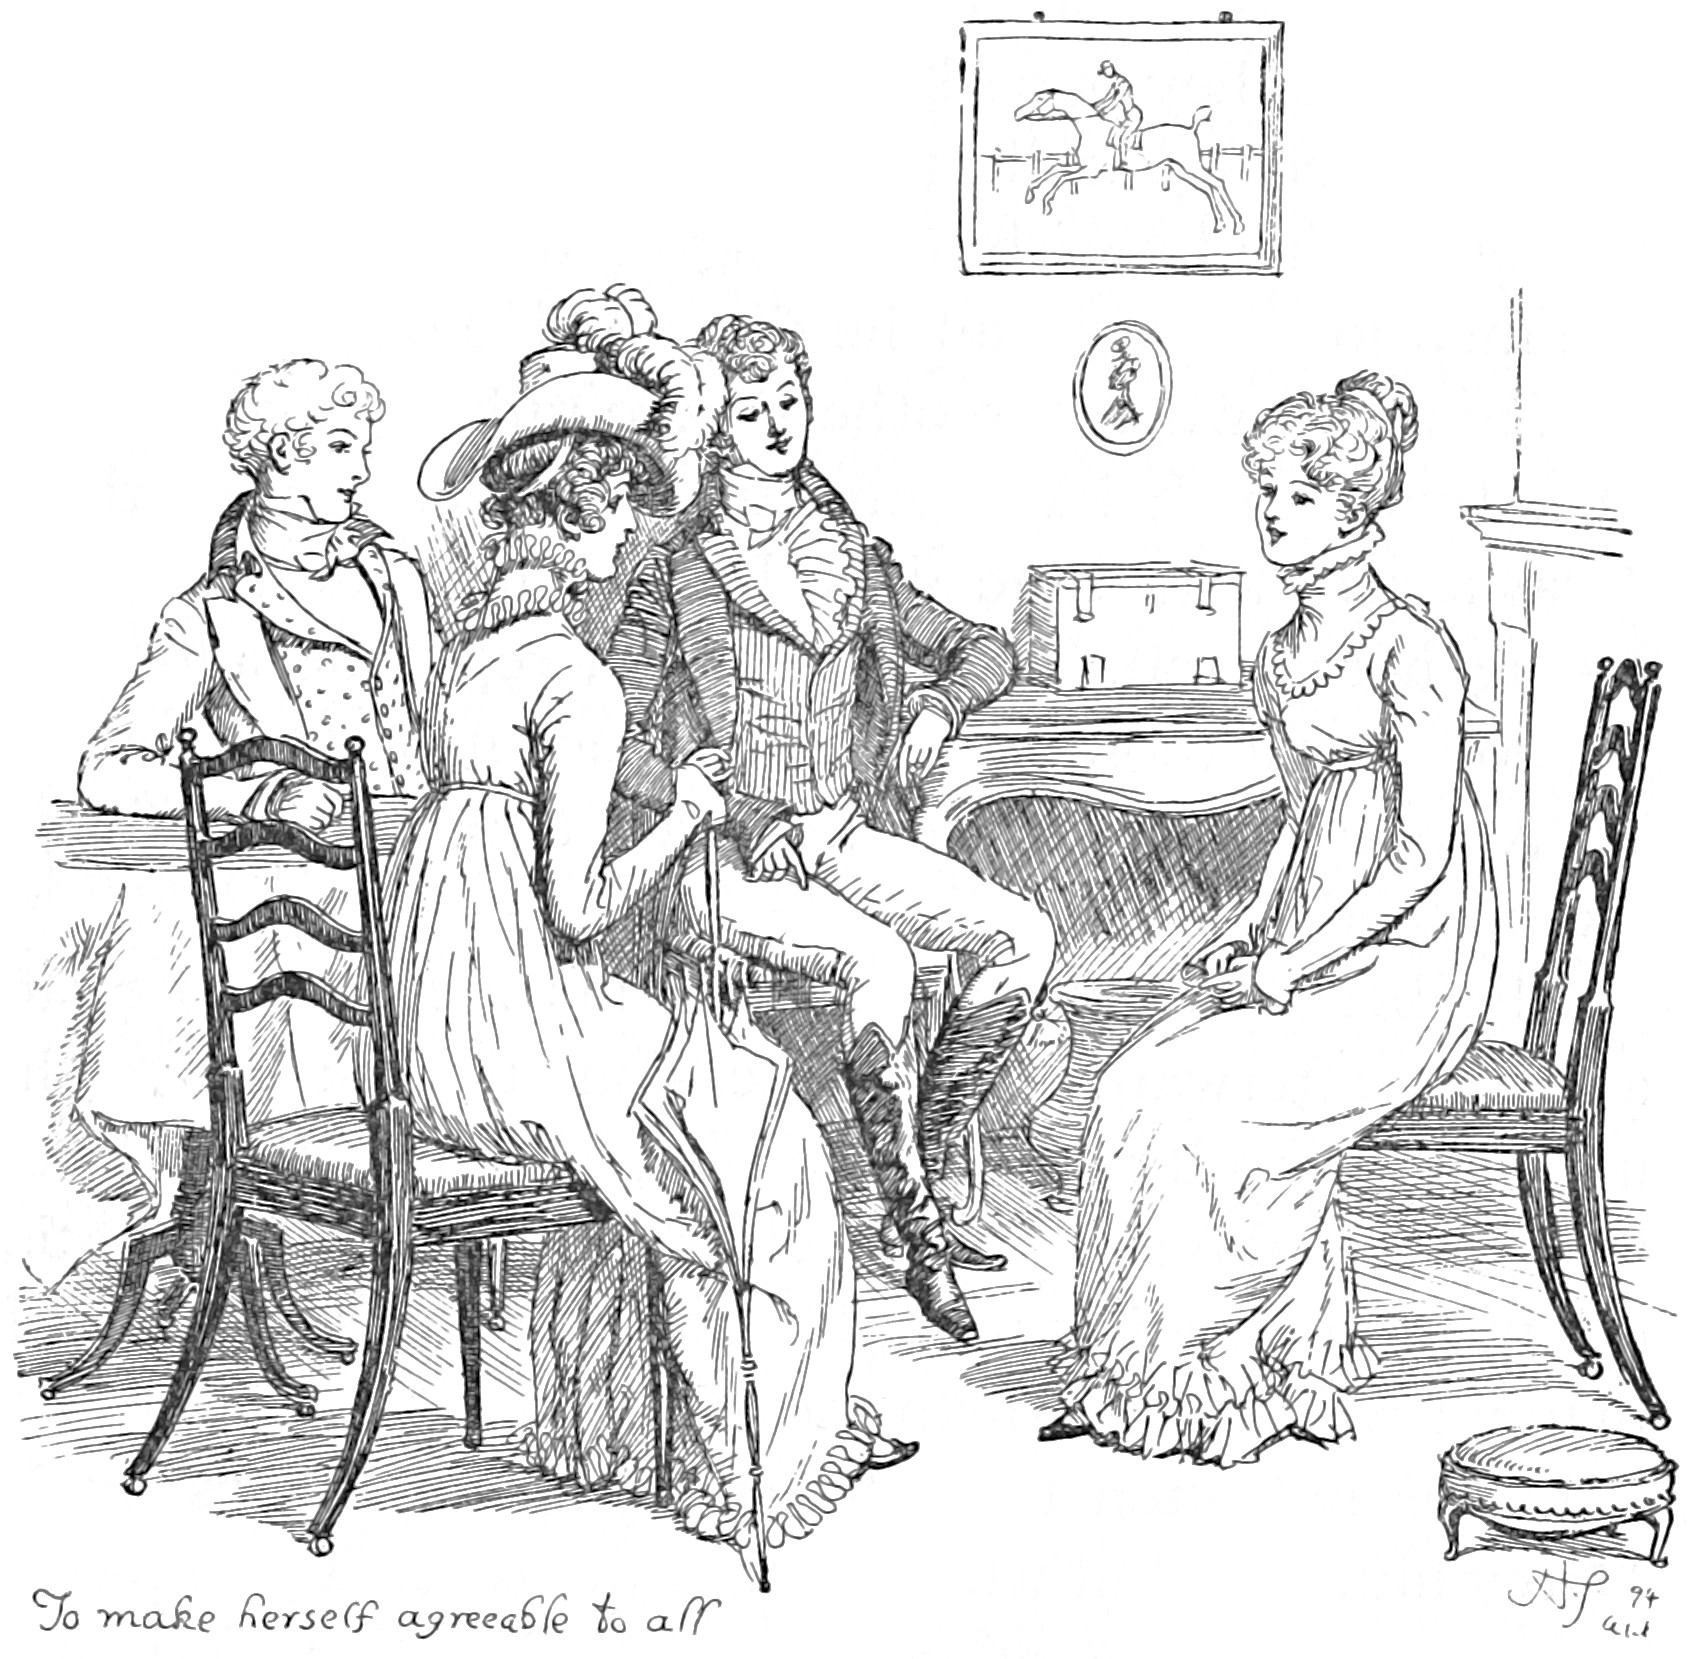
\includegraphics[width=.8\linewidth]{44agreeable}
\captionlistentry{To make herself agreeable to all}
\end{figure}

Elizabeth, on her side, had much to do. She wanted to ascertain the feelings of each of her visitors, she wanted to compose her own, and to make herself agreeable to all; and in the latter object, where she feared most to fail, she was most sure of success, for those to whom she endeavoured to give pleasure were pre-possessed in her favour. Bingley was ready, Georgiana was eager, and Darcy determined, to be pleased.

In seeing Bingley, her thoughts naturally flew to her sister; and oh! how ardently did she long to know whether any of his were directed in a like manner. Sometimes she could fancy that he talked less than on former occasions, and once or twice pleased herself with the notion that, as he looked at her, he was trying to trace a resemblance. But, though this might be imaginary, she could not be deceived as to his behaviour to Miss Darcy, who had been set up as a rival to Jane. No look appeared on either side that spoke particular regard. Nothing occurred between them that could justify the hopes of his sister. On this point she was soon satisfied; and two or three little circumstances occurred ere they parted, which, in her anxious interpretation, denoted a recollection of Jane, not untinctured by tenderness, and a wish of saying more that might lead to the mention of her, had he dared. He observed to her, at a moment when the others were talking together, and in a tone which had something of real regret, that it »was a very long time since he had had the pleasure of seeing her;« and, before she could reply, he added, »It is above eight months. We have not met since the 26th of November, when we were all dancing together at Netherfield.«

Elizabeth was pleased to find his memory so exact; and he afterwards took occasion to ask her, when unattended to by any of the rest, whether \textit{all} her sisters were at Longbourn. There was not much in the question, nor in the preceding remark; but there was a look and a manner which gave them meaning.

It was not often that she could turn her eyes on Mr Darcy himself; but whenever she did catch a glimpse she saw an expression of general complaisance, and in all that he said, she heard an accent so far removed from \textit{hauteur} or disdain of his companions, as convinced her that the improvement of manners which she had yesterday witnessed, however temporary its existence might prove, had at least outlived one day. When she saw him thus seeking the acquaintance, and courting the good opinion of people with whom any intercourse a few months ago would have been a disgrace; when she saw him thus civil, not only to herself, but to the very relations whom he had openly disdained, and recollected their last lively scene in Hunsford Parsonage, the difference, the change was so great, and struck so forcibly on her mind, that she could hardly restrain her astonishment from being visible. Never, even in the company of his dear friends at Netherfield, or his dignified relations at Rosings, had she seen him so desirous to please, so free from self-consequence or unbending reserve, as now, when no importance could result from the success of his endeavours, and when even the acquaintance of those to whom his attentions were addressed, would draw down the ridicule and censure of the ladies both of Netherfield and Rosings.

Their visitors stayed with them above half an hour; and when they arose to depart, Mr Darcy called on his sister to join him in expressing their wish of seeing Mr and Mrs Gardiner, and Miss Bennet, to dinner at Pemberley, before they left the country. Miss Darcy, though with a diffidence which marked her little in the habit of giving invitations, readily obeyed. Mrs Gardiner looked at her niece, desirous of knowing how \textit{she}, whom the invitation most concerned, felt disposed as to its acceptance, but Elizabeth had turned away her head. Presuming, however, that this studied avoidance spoke rather a momentary embarrassment than any dislike of the proposal, and seeing in her husband, who was fond of society, a perfect willingness to accept it, she ventured to engage for her attendance, and the day after the next was fixed on.

Bingley expressed great pleasure in the certainty of seeing Elizabeth again, having still a great deal to say to her, and many inquiries to make after all their Hertfordshire friends. Elizabeth, construing all this into a wish of hearing her speak of her sister, was pleased; and on this account, as well as some others, found herself, when their visitors left them, capable of considering the last half hour with some satisfaction, though while it was passing the enjoyment of it had been little. Eager to be alone, and fearful of inquiries or hints from her uncle and aunt, she stayed with them only long enough to hear their favourable opinion of Bingley, and then hurried away to dress.

But she had no reason to fear Mr and Mrs Gardiner's curiosity; it was not their wish to force her communication. It was evident that she was much better acquainted with Mr Darcy than they had before any idea of; it was evident that he was very much in love with her. They saw much to interest, but nothing to justify inquiry.

Of Mr Darcy it was now a matter of anxiety to think well; and, as far as their acquaintance reached, there was no fault to find. They could not be untouched by his politeness; and had they drawn his character from their own feelings and his servant's report, without any reference to any other account, the circle in Hertfordshire to which he was known would not have recognized it for Mr Darcy. There was now an interest, however, in believing the housekeeper; and they soon became sensible that the authority of a servant, who had known him since he was four years old, and whose own manners indicated respectability, was not to be hastily rejected. Neither had anything occurred in the intelligence of their Lambton friends that could materially lessen its weight. They had nothing to accuse him of but pride; pride he probably had, and if not, it would certainly be imputed by the inhabitants of a small market town where the family did not visit. It was acknowledged, however, that he was a liberal man, and did much good among the poor.

With respect to Wickham, the travellers soon found that he was not held there in much estimation; for though the chief of his concerns with the son of his patron were imperfectly understood, it was yet a well-known fact that, on his quitting Derbyshire, he had left many debts behind him, which Mr Darcy afterwards discharged.

As for Elizabeth, her thoughts were at Pemberley this evening more than the last; and the evening, though as it passed it seemed long, was not long enough to determine her feelings towards \textit{one} in that mansion; and she lay awake two whole hours, endeavouring to make them out. She certainly did not hate him. No; hatred had vanished long ago, and she had almost as long been ashamed of ever feeling a dislike against him, that could be so called. The respect created by the conviction of his valuable qualities, though at first unwillingly admitted, had for some time ceased to be repugnant to her feelings; and it was now heightened into somewhat of a friendlier nature by the testimony so highly in his favour, and bringing forward his disposition in so amiable a light, which yesterday had produced. But above all, above respect and esteem, there was a motive within her of good-will which could not be overlooked. It was gratitude;—gratitude, not merely for having once loved her, but for loving her still well enough to forgive all the petulance and acrimony of her manner in rejecting him, and all the unjust accusations accompanying her rejection. He who, she had been persuaded, would avoid her as his greatest enemy, seemed, on this accidental meeting, most eager to preserve the acquaintance; and without any indelicate display of regard, or any peculiarity of manner, where their two selves only were concerned, was soliciting the good opinion of her friends, and bent on making her known to his sister. Such a change in a man of so much pride excited not only astonishment but gratitude—for to love, ardent love, it must be attributed; and, as such, its impression on her was of a sort to be encouraged, as by no means unpleasing, though it could not be exactly defined. She respected, she esteemed, she was grateful to him, she felt a real interest in his welfare; and she only wanted to know how far she wished that welfare to depend upon herself, and how far it would be for the happiness of both that she should employ the power, which her fancy told her she still possessed, of bringing on the renewal of his addresses.

It had been settled in the evening, between the aunt and niece, that such a striking civility as Miss Darcy's, in coming to them on the very day of her arrival at Pemberley—for she had reached it only to a late breakfast—ought to be imitated, though it could not be equalled, by some exertion of politeness on their side; and, consequently, that it would be highly expedient to wait on her at Pemberley the following morning. They were, therefore, to go. Elizabeth was pleased; though when she asked herself the reason, she had very little to say in reply.

Mr Gardiner left them soon after breakfast. The fishing scheme had been renewed the day before, and a positive engagement made of his meeting some of the gentlemen at Pemberley by noon.